\chapter{Controlling Weakly-coupled Carbon Spins}
[Note intro needs to be rewritten once chapter is done]\\
Now that we have identified several promising carbon spins we will go into controlling them.
This chapter attempts to explain first how we can control a carbon by explaining how the two different rotation axes from the last chapter can be used to implement a conditional +-X gate. A gate similar to a CNOT gate.
Now that we understand how to implement a cnot gate we will use this to perform an experiment that we call a carbon ramsey on an unitialized state.
AFterwards we will use this to show that we can initialize and readout by showing an initialized carbon ramsey. (1buit tomo (ramsey with more T +Z-RO?).
From this we will also determine $T_{2 \mathrm{C}}^*$.

The next section will consider two qubit control.
It will start by explaining how we can perform a parity measurement. This measurement allows us to perform a two qubit tomography and create entanglement by projection.
We will then show

\section{Controlling a single-carbon}
This section will explain how a weakly-coupled spin can be controlled using the conditional rotation of the carbon spin that occurs when on resonance (\cref{eq:res_dip_loc}).
It will start by explaining how to do basic gate operations in the ideal case of being perfectly on resonant and not interacting with any nuclear spins.
After that we will explain

\subsection{Carbon Rabi?}

\subsection{Basic gates}
As was explained in section \cref{controllingacarbonthroughdynamicaldecoupling}
\begin{figure}[htbp]
    \begin{subfigure}[t]{0.49\textwidth}
    \centering
        \mbox{
        \Qcircuit @C=1em @R=.7em {
         \lstick{\ket{\Psi}_e} &\ctrl{1}  &\qw\\
          \lstick{\ket{\Psi}_\mathrm{C}} &\gate{\pm \mathrm{x} }  &\qw}}
        \caption{The conditional x-gate ($\pm\mathrm{x}$).}
        \label{fig:gate_circuit_pm-x}
    \end{subfigure}
    \begin{subfigure}[t]{0.49\textwidth}
        \centering
        \mbox{
        \Qcircuit @C=1em @R=.7em {
          &\ctrl{1}  &\qw &\dstick{=} &&\qw& \ctrl{1} &\qw \\
          &\gate{\pm \mathrm{y} }  &\qw &&& \gate{\mathrm{z}}  &\gate{\pm \mathrm{x} } &\qw}}
        \caption{The conditional y-gate ($\pm\mathrm{y}$) is implemented by letting the phase evolve before performing a conditional x rotation ($\pm\mathrm{x}$) on the carbon.}
        \label{fig:gate_circuit_carbon_phase}
    \end{subfigure}
    \label{fig:basic_carbon_gates}
    \caption{\Cref{fig:gate_circuit_pm-x} The conditional x-gate ($\pm\mathrm{x}$). Performs an x-rotation on the carbon state ($\ket{\Psi }_C$) when the electron is in the $\ket{0}_e$-state. It performs a $-\mathrm{x}$ rotation when the electron is in the $\ket{1}_e$-state. \Cref{fig:gate_circuit_carbon_phase} Phases in carbon gates are implemented by letting the phase of the carbon evolve before applying a conditional x-gate.}
\end{figure}

\subsubsection{$\pm$x gate }
\subsubsection{An unconditional gate }
\subsubsection{A phase gate}

\subsection{Addressing an uninitialized carbon (carbon Ramsey) }
\subsubsection{Theory, what happens if }
\subsubsection{Experiment}

\subsection{Controlling a single carbon}
\subsubsection{Theory, initialization and readout}
\subsubsection{Single qubit tomography and T2*}

\section{Controlling multiple-carbons}
\subsection{The parity measurement}
\subsection{MBE}


When on resonance (\cref{eq:res_dip_loc} ) the carbon rotates around on of two distinct anti-parallel axes based on the state the electron is in.
[Need some statement that puts the axis in the equator when on resonance. Look in appendix again ]
We define the

Figure of Bloch sphere whoing n0 and n1 axis.
A state starting of in 0 being rotated to +y and -y ($\pm $ x operation).
Different arrow


adf

\subsection{Carbon Ramsey experiment }



\subsection{Measuring Precession Frequencies/Carbon Ramsey experiment}
% Ramsey experiment to measure coupling strengths
% Needs relation between frequency and parralel component
% spins 1 and 4 best
Idea explain init with swap init. And from there go back to X-init. Refer to appendix for more rigorous derivation.


\begin{figure}[htbp]
    \centering
\mbox{
\Qcircuit @C=1em @R=.7em {
\lstick{\ket{0}}          & \gate{\pi/2}  & \ctrl{1}      & \qw & \multigate{1}{T}       &  \qw &\ctrl{1}          & \gate{\pi/2} &\qw          &  \meter \\
\lstick{\rho_\mathrm{m}}         & \qw              &  \gate{\pm \mathrm{x}}     & \qw& \ghost{T}        & \qw & \gate{\pm \mathrm{x}}      & \qw       &\qw&}}
    \caption{Carbon Ramsey experiment. }
    \label{fig:gate_circuit_nuclear_ramsey}
\end{figure}

\begin{figure}[htbp]
    \centering
\mbox{
\Qcircuit @C=1em @R=.7em {
\lstick{\ket{0}_e}                        & \gate{\mathrm{y}}  & \ctrl{1}       & \gate{x} &\qw          &  \meter &\qw\\
\lstick{\rho_\mathrm{m}}         & \qw              &  \gate{\pm \mathrm{x}}     & \qw    & \qw   & \qw       &\qw&}}
    \caption{MBI-based initialization into $\pm \ket{\mathrm{X}}$. Initializes the carbon into $\ket{X}_C $ when $\ket{0}_e$ is measured and into $\ket{-X}_C $ when $\ket{1}_e$ is measured for the electron.}
    \label{fig:gate_circuit_mbi_x-init}
\end{figure}

\begin{figure}[htbp]
    \centering
\mbox{
\Qcircuit @C=1em @R=.7em {
\lstick{\ket{0}_e} & \gate{\mathrm{y}}  & \ctrl{1} & \gate{x} &\ctrl{1} &  \meter &\qw\\
\lstick{\rho_\mathrm{m}}& \qw&  \gate{\pm \mathrm{x}}     & \qw    & \gate{\pm \mathrm{y}}    & \qw       &\qw&}}
    \caption{MBI-swap initialization into $\pm \ket{\mathrm{0}}$. Initializes the carbon into $\ket{0}_C $ when $\ket{0}_e$ is measured and into $\ket{1}_C $ when $\ket{1}_e$ is measured for the electron.}
    \label{fig:gate_circuit_mbi_swap-init}
\end{figure}


\begin{figure}[htbp]
    \centering
\mbox{
\Qcircuit @C=1em @R=.7em {
\lstick{\ket{0}_e} & \gate{\mathrm{y}}  & \ctrl{1} &  \ctrl{2} & \gate{y}  &  \meter &\qw\\
\lstick{\ket{0}_{C1}} & \qw&  \gate{\pm \mathrm{x}}  &\qw  & \qw       &\qw&\qw& \\
\lstick{\ket{0}_{C2}}& \qw& \qw  & \gate{\pm \mathrm{x}}    & \qw      &\qw&\qw&}}
    \caption{XX-parity-measurement}
    \label{fig:gate_circuit_XX-parity-measurement}
\end{figure}

\begin{figure}[htbp]
    \centering
\mbox{
\Qcircuit @C=1em @R=.7em {
\lstick{\ket{0}_e} & \gate{\mathrm{y}}  & \ctrl{1} &  \ctrl{2} & \gate{\mathrm{y}}  & \ctrl{1} &  \ctrl{2} &  \meter &\qw\\
\lstick{\ket{0}_{C1}} & \qw&  \gate{\pm \mathrm{x}}  &\qw  &\qw  & \gate{\pm \mathrm{x}} & \qw   &\qw&\qw& \\
\lstick{\ket{0}_{C2}}& \qw& \qw  & \gate{\pm \mathrm{x}}    & \qw    &\qw& \gate{\pm \mathrm{x}}    & \qw &\qw&}}
    \caption{General parity RO}
    \label{fig:gate_circuit_general_Parity_RO}
\end{figure}


\begin{figure}[htbp]
    \begin{subfigure}[t]{0.49\textwidth}\centering
    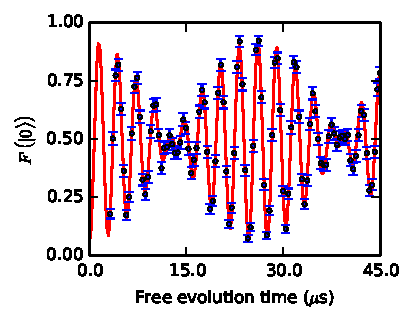
\includegraphics{Img/CarbonRamsey_C1.pdf}
    \caption{Nuclear Ramsey of Carbon 1} \label{fig:CR_C1}
    \end{subfigure}
    \begin{subfigure}[t]{0.49\textwidth}\centering
        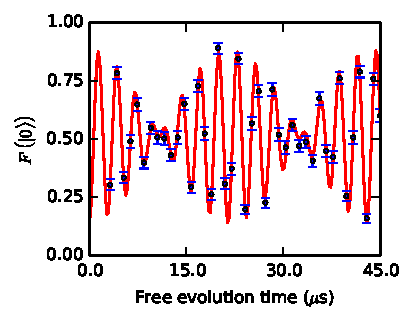
\includegraphics{Img/CarbonRamsey_C4.pdf}
        \caption{Nuclear Ramsey of Carbon 4}
        \label{fig:CR_C4}
    \end{subfigure}
    \caption{Nuclear Ramsey experiment wit}
\end{figure}



\section{Controlling weakly coupled carbons trough the electronic spin}
% Section containing theory (Gate circuits) on how to initialize and readout carbons

Explain how carbon control works in theory.
Explain how a conditional and unconditional gate can be performed.
Explain initialization on gate level, refer to appendix for calculations.
Explain Readout.

\subsection{Initialized Carbon Ramsey}


\section{Carbon Initialization \& Readout}
% TODO_MAR: Discuss naming of sec: Carbon Init&RO and Carbon Tomo
%  Section containing experimental results (Tomographies)
%  Should emphasize difficulty in seperating initialization and RO fidelity, what is not working? Is it working?
Show results that demonstrate carbon control.



